\chapter{Desarrollo del entorno base}\label{ch:desarrollo-del-entorno-base}

En este capítulo se abordará el desarrollo de la aplicación base, empezando por la investigación
de tecnologías.
También se definirá la estructura final de la aplicación en los ámbitos de la interfaz y el código.


\section{Definición de los requisitos de las tecnologías candidatas}
\label{sec:definicion-requisitos-tecnologías-candidatas}

Actualmente, existe una gran variedad de librerías y \textit{frameworks} gráficos que permiten
crear aplicaciones de una manera rápida y sencilla.
Estas tecnologías se pueden clasificar dependiendo de una gran cantidad de criterios.

\noindent Según su nivel de abstracción:
\begin{itemize}
    \item \textbf{Librerías de bajo nivel:} son más cercanas al \textit{hardware} gráfico.
    Permiten tener un gran control sobre los gráficos, pero no son adecuadas para
    interfaces gráficas de usuarios.
    Algunos ejemplos de librerías de bajo nivel son \textit{OpenGL}, \textit{Vulkan} o \textit{DirectX}.
    \item \textbf{Librerías de alto nivel}: incorporan una capa de abstracción sobre el \textit{hardware} gráfico.
    Permiten generar interfaces gráficas de usuario mediante una arquitectura ya definida.
    Algunos ejemplos de librerías de alto nivel son \textit{Qt}, \textit{JavaFX}, \textit{Swing}, \textit{GTK} o
    \textit{Compose Multiplatform}.
\end{itemize}

\noindent Según su disponibilidad en varias plataformas:
\begin{itemize}
    \item \textbf{Librerías exclusivas:} son librerías que solo están disponibles en una plataforma.
    Algunos ejemplos de librerías exclusivas son \textit{Windows Forms} y \textit{DirectX} en \textit{Windows},
    \textit{Metal} y \textit{QuickDraw} en \textit{MacOS} o \textit{AndroidX/Graphics} y \textit{Jetpack Compose}
    en \textit{Android}.
    \item \textbf{Librerías multiplataforma:} están disponibles en una gran variedad de plataformas.
    Algunos ejemplos de librerías multiplataforma son \textit{Qt}, \textit{JavaFX}, \textit{Swing}, \textit{GTK}
    o \textit{Compose Multiplatform}.
\end{itemize}

\noindent Un aspecto muy importante al elegir candidatos es el \textbf{lenguaje de programación}
en el que las librerías están disponibles.
Las librerías de bajo nivel suelen estar disponibles en una gran variedad de lenguajes, mientras que las
librerías de alto nivel suelen incorporar paradigmas propios del lenguaje de programación en el que están
desarrolladas.

\noindent Para el desarrollo de la aplicación se desea utilizar una librería gráfica \textbf{moderna},
\textbf{de alto nivel} y \textbf{multiplataforma}, disponible en un lenguaje de programación estable,
con una comunidad grande y \textbf{rápido tanto en el desarrollo como en la ejecución}.
Otro requisito crucial es que el lenguaje permita \textbf{vincular código externo} de manera
sencilla.

\noindent Estos requisitos reduce la lista de tecnologías en los siguientes candidatos:
\begin{itemize}
    \item \textbf{HTML, CSS y TypeScript:} este conjunto de tecnologías es muy popular actualmente
    para la creación de aplicaciones web y de escritorio. \textit{IDEs} muy famosos como
    \textit{Visual Studio Code} están desarrollados con estas tecnologías.
    \item \textbf{Kotlin / Compose Multiplatform:} \textit{Compose Multiplatform} es una librería gráfica
    para \textit{Kotlin}, un lenguaje de programación muy joven y potente que tiene el respaldo de
    grandes compañías como \textit{JetBrains} y \textit{Google}.
    \item \textbf{Java / JavaFX:} \textit{JavaFX} puede considerarse la evolución natural de \textit{Swing},
    la herramienta principal para el desarrollo de aplicaciones gráficas basadas en \textit{Java}.
    \textit{JavaFX} es una librería moderna y rápida que, gracias a que está desarrollada en \textit{Java},
    puede ser empleada por otros lenguajes de programación que corren sobre la \textit{JVM}
    \footnote{\textit{Java Virtual Machine}}, como es el caso de \textit{Scala}, \textit{Groovy} o el ya mencionado
    \textit{Kotlin}.
\end{itemize}

\noindent El trío \textit{HTML / CSS / TypeScript} suele ser una buena elección para editores y otras
aplicaciones ligeras, pero la falta de velocidad en la ejecución y la falta de consistencia por estar
basado \textit{TypeScript} en \textit{JavaScript} descarta esta opción por parte del simulador.

\noindent \textit{Kotlin / Compose Multiplatform} es una elección muy sólida actualmente, pero esta
tecnología seguía en fase \textit{beta} cuando este proyecto empezó, por lo que también ha quedado
descartada.

\noindent Finalmente, \textbf{se ha optado por utilizar el par de tecnologías \textit{Java / JavaFX}}
para el desarrollo de la aplicación, ya que cumple con todos los requisitos: \textit{Java} es un
lenguaje de programación muy estable, multiplataforma y rápido tanto en la ejecución como en
el desarrollo.
También es el lenguaje de programación con la comunidad de desarrolladores más grande.
\textit{JavaFX} es una alternativa moderna a \textit{Swing} que permite desarrollar aplicaciones
fácilmente personalizables que se alejan del ya conocido estilo de interfaz \textit{Java}.

\noindent Centrándose en otras tecnologías necesarias, se ha utilizado el entorno de desarrollo
\textit{Intellij IDEA} y el sistema de automatización \textit{Gradle} para la construcción
del proyecto.

\subsection{En defensa de \textit{Java}}\label{subsec:en-defensa-de-java}

Muchos desarrolladores piensan que \textit{Java} es un lenguaje de programación verboso, lento, pesado
y con el único propósito de crear aplicaciones \textit{Spring}.
Que la mayoría de aplicaciones \textit{Java} estén desarrolladas en versiones \textit{vanilla}
\footnote{Estándar, sin modificar} de \textit{Swing} y en versiones de \textit{Java} de hace más
de un lustro no ayuda en su reputación.

\noindent La realidad es muy diferente: su equipo de desarrollo lleva años reinventando su tecnología,
con nuevas características que acercan a \textit{Java} a lenguajes de programación mucho más modernos.
La velocidad de ejecución también se ha incrementado considerablemente, posicionándose en uno de los
lenguajes de programación que más rápido ejecutan.

\noindent Un gran ejemplo del drástico cambio que ha sufrido \textit{Java} en los últimos años son los
\textit{records}: clases de datos que son inmutables.

\begin{lstlisting}[language=Java,style=java,frame=single,label={lst:java-comparacion-18}]
public record Cat(String name, UUID owner) {
}
\end{lstlisting}

\noindent El código equivalente en \textit{Java} 8 sería el siguiente:

\begin{lstlisting}[language=Java,style=java,frame=single,label={lst:java-comparacion-8}]
public final class Cat {
    private final String name;
    private final UUID owner;

    public Cat(String name, UUID owner) {
        this.name = name;
        this.owner = owner;
    }

    public String name() { return name; }

    public UUID owner() { return owner; }

    @Override
    public boolean equals(Object obj) {
        if (obj == this) return true;
        if (obj == null || obj.getClass() != this.getClass()) return false;
        var that = (Cat) obj;
        return Objects.equals(this.name, that.name) &&
                Objects.equals(this.owner, that.owner);
    }

    @Override
    public int hashCode() { return Objects.hash(name, owner); }

    @Override
    public String toString() { return "Cat[" + "name=" + name
        + ", " + "owner=" + owner + ']'; }

}
\end{lstlisting}

\noindent La nueva arquitectura basada en módulos que presenta las librerías de \textit{Java}
ayuda mucho en la distribución de aplicaciones de escritorio, pudiendo generar un instalador
convencional que instala la aplicación junto con una versión local de la \textit{JVM} que no
suele superar los 30 MB\cite{JPACKAGE}.
Gracias a este sistema de distribución, la aplicación podrá contar con versiones
de \textit{Java} actuales sin que los usuarios tengan que pasar por complejas instalaciones.

\noindent Como dato final, existen muchas aplicaciones que se ejecutan sobre la \textit{JVM}
sin que el usuario se de cuenta.
Este es el caso de todos los \textit{IDEs} desarrollados por \textit{JetBrains}, los cuales
usan la librería \textit{Swing} con un estilo avanzado.

\begin{figure}[H]
    \centering
    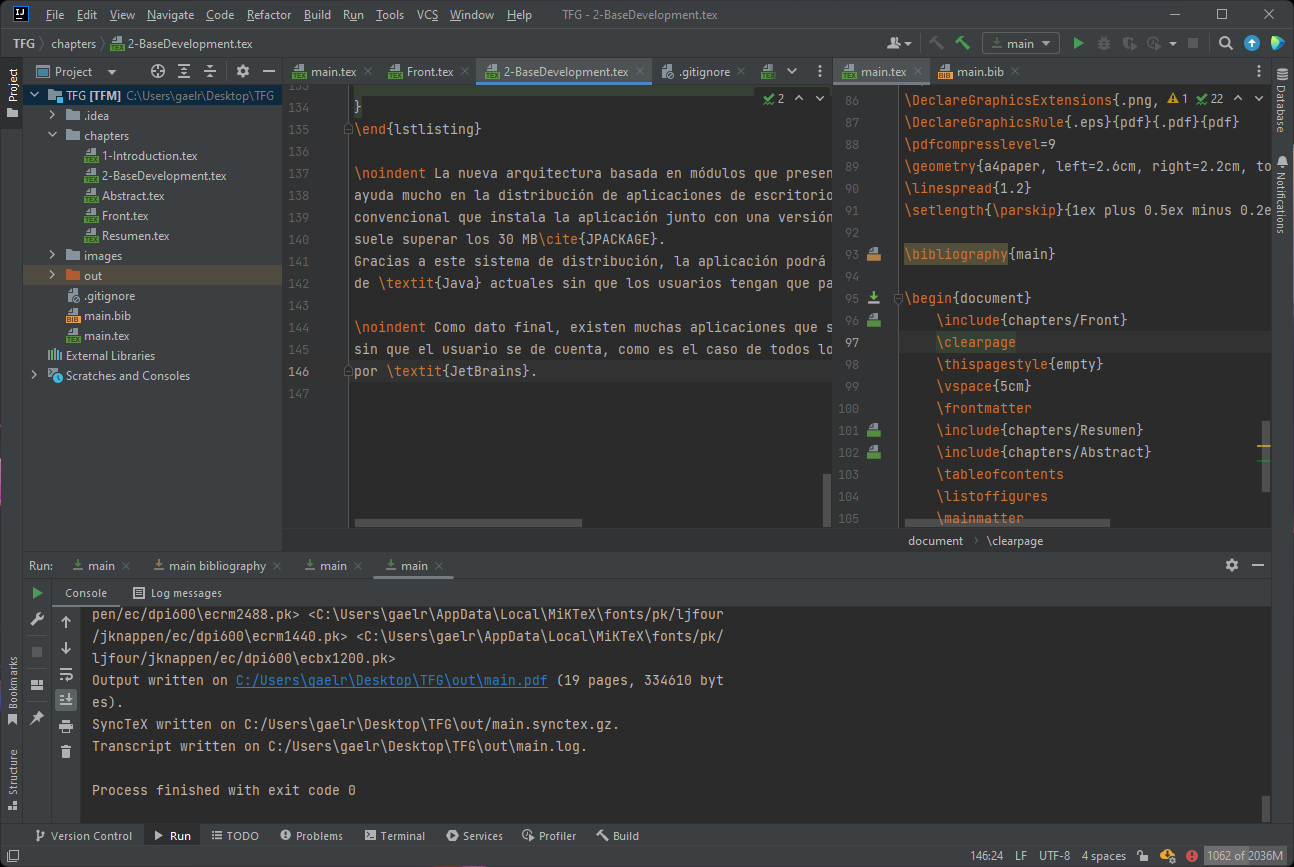
\includegraphics[width=\textwidth]{images/base/intellij-idea}
    \caption{\textit{Intellij IDEA}}
    \label{fig:java-intellij-idea}
\end{figure}


\section{Estructura del proyecto}\label{sec:estructura-del-proyecto}

\textit{JAMS} sigue los estándares de estructura de \textit{Gradle}\cite{GRADLE_ORGANIZING}.
Esto hace que su estructura sea muy similar a otras aplicaciones que usan el mismo
sistema de automatización.

\subsection{Tareas}\label{subsec:tareas}

\noindent El elemento más importante del directorio raíz es el archivo \textbf{build.gradle}.
En él se especifican las dependencias y se define cómo el proyecto debe ser compilado.
Las \textbf{tareas} son las encargadas de definir dicho comportamiento.

\noindent Las dos tareas más importantes son las siguientes:
\begin{itemize}
    \item \textbf{jpackage:} permite generar un instalador de la aplicación específico
    para la máquina que ejecuta la tarea.
    \item \textbf{bundle:} genera un archivo \textit{jar} con la aplicación y todas
    sus dependencias.
    Este archivo puede ser ejecutado en cualquier sistema operativo que pueda correr
    \textit{Java} y esté soportado por \textit{JavaFX}.
\end{itemize}

\noindent Para ejecutar estas tareas ha de usarse el \textit{script} \textbf{gradlew}.
Este comando descargará \textit{Gradle} si es necesario y ejecutará
la tarea pasada como argumento.
Todos estos comportamientos están automatizados en \textit{GitHub}
mediante los \textit{scripts} dentro de la carpeta \textbf{.github}.

\subsection{Módulos y paquetes}\label{subsec:modulos-y-paquetes}

Dentro de la carpeta \textbf{src} están definidos los dos módulos principales del
proyecto: \textbf{main} y \textbf{test}.

\noindent El módulo \textbf{main} es el encargado de almacenar todo el código fuente
de la aplicación.
Puede ser considerado el módulo más importante de todo el proyecto.
El módulo \textbf{test} define todas las pruebas unitarias que el módulo \textbf{main}
debe superar para que la aplicación se compile con éxito.

\noindent El código fuente almacenado en el módulo \textbf{main} está separado en diferentes
paquetes \textit{Java}:
\begin{itemize}
    \item \textbf{collection:} contiene una serie de colecciones modificadas.
    \item \textbf{configuration:} contiene el sistema de configuraciones.
    \item \textbf{event:} contiene el sistema de eventos.
    \item \textbf{file:} contiene los tipos de archivo definidos en la aplicación.
    \item \textbf{gui:} contiene toda la interfaz de la aplicación.
    \item \textbf{language:} contiene el sistema de idiomas.
    \item \textbf{manager:} contiene el sistema de gestores.
    \item \textbf{mips:} contiene todas las herramientas relacionadas con la arquitectura \textit{MIPS32}.
    \item \textbf{plugin:} contiene el sistema de componentes.
    \item \textbf{project:} contiene el sistema de proyectos.
    \item \textbf{task:} contiene el sistema de hijos y tareas asíncronas.
    \item \textbf{utils:} contiene clases útiles utilizadas por los anteriores paquetes.
\end{itemize}


\section{Proyectos}\label{sec:interfaz-grafica}

\textit{JAMS} es un \textit{IDE} basado en \textbf{proyectos}.
Un proyecto está formado por una carpeta y las siguientes propiedades:
\begin{itemize}
    \item \textbf{Tipo de proyecto:} especifica el tipo de proyecto.
    En una versión sin componentes este valor solo puede tomar el valor \textit{MIPS}.
    \item \textbf{Propiedades del proyecto:} parámetros necesarios por el tipo de proyecto.
    Configuran aspectos concretos y generales de todo el proyecto.
    \item \textbf{Archivos a ensamblar:} lista de archivos que el ensamblador tendrá en cuenta
    al ensamblar el proyecto.
    \item \textbf{Configuraciones:} especifican propiedades \textbf{de una ejecución} del proyecto.
    Es decir, configuran el simulador.
    Un proyecto puede tener varias configuraciones, y el usuario ha de elegir una al crear una
    simulación.
\end{itemize}

\noindent Los proyectos son almacenados en carpetas.
Una carpeta de un proyecto tiene la siguiente estructura:

\begin{center}
    \basictree{
        [MyProject
        [.jams
        [data.json]
        [files\_to\_assemble.json]
        ]
        [Simulation Files
        [MySimulationFile.txt]
        ]
        [MyAsmFile.asm]
        ]
    }
\end{center}

\noindent Cada proyecto tiene dos carpetas por defecto: \textbf{.jams} y
\textbf{Simulation Files}.
La carpeta \textbf{.jams} contiene los datos del proyecto que \textit{JAMS}
gestiona de manera automática.
Esta carpeta está oculta y no debe ser modificada por el usuario.
El archivo \textbf{data.json} contiene el tipo de proyecto y sus propiedades,
mientras que \textit{files\_to\_assemble.json} contiene la listas de archivos
que el ensamblador ha de usar.
La carpeta \textit{Simulation Files} actúa de carpeta raíz del simulador:
todos los archivos que escriba o lea el simulador deben estar situados dentro
de esta carpeta.


\section{Gestores}\label{sec:gestores}

Toda la arquitectura de la aplicación está basada en \textbf{gestores}.
Un gestor se puede definir como un conjunto de elementos que las herramientas pueden usar.
\textit{JAMS} proporciona tres tipos básicos de gestores:
\begin{itemize}
    \item \textbf{Gestores normales:} implementados por la clase \textit{Manager}.
    Contienen una lista de elementos sin ninguna jerarquía.
    \item \textbf{Gestores con valor por defecto:} actúa como un gestor normal, con la
    diferencia que uno de sus valores es el valor por defecto.
    Estos gestores heredan de la clase \textit{DefaultValuableManager}.
    \item \textbf{Gestores con valor seleccionado:} actúan como un gestor con valor por defecto,
    pero con uno de los elementos seleccionado.
    Cuando el elemento seleccionado se elimina, el elemento por defecto queda seleccionado.
    Estos gestores heredan de la clase \textit{SelectableManager}.
\end{itemize}

\subsection{Proveedores}\label{subsec:proveedores}

Cada elemento guardado en un gestor \textbf{está asociado al proveedor que lo proporciona}.
Un proveedor puede ser un plugin o el propio \textit{JAMS}.
Cuando un proveedor se desvincula de la aplicación, todos los elementos proporcionados
por el proveedor son eliminados de los gestores.

\subsection{Registro}\label{subsec:registro}

El registro es un \textbf{elemento estático dentro de la aplicación}.
Se puede considerar un \textbf{gestor de gestores}.
En el registro se pueden recuperar, añadir, eliminar o modificar gestores.
Igual que los gestores normales, cuando un proveedor se desvincula de la aplicación,
todos los gestores proporcionados por el proveedor son eliminados del registro.

\noindent \textit{JAMS} permite separar los gestores en dos tipos:
\textbf{gestores primarios} y \textbf{gestores secundarios}.
Los gestores primarios son fácilmente accesibles cuando se busca un gestor por tipo
usando métodos como \textbf{Manager.of(Type.class)}.
Solo puede existir un gestor primario por tipo.
Para buscar gestores secundarios, se debe proveer el nombre del gestor explícitamente.

\subsection{Acceder a los gestores}\label{subsec:acceder-a-los-gestores}

Existen dos maneras de acceder a un gestor: \textbf{usando el registro} o
\textbf{usando los atajos de la clase Manager}.

\begin{lstlisting}[language=Java,style=java,frame=single,label={lst:acceder-a-los-gestores}]
// Returns the primary manager that manages languages.
Manager<Language> simpleLanguageManager = Manager.of(Language.class);
simpleLanguageManager = Jams.REGISTRY.of(Language.class);

// Returns the primary selectable manager that manages languages.
SelectableManager<Language> selectableLanguageManager = Manager.ofS(Language.class);
selectableLanguageManager = (SelectableManager<Language>) Jams.REGISTRY.of(Language.class);

// Returns the manager that is an instance of LanguageManager.
LanguageManager languageManager = Manager.get(LanguageManager.class);
languageManager = Jams.REGISTRY.get(LanguageManager.class);

// Returns the manager with the given name.
Manager<Language> manager = Jams.REGISTRY.of("other-language-manager", Language.class);
\end{lstlisting}

\subsection{Usar los gestores}\label{subsec:usar-los-gestores}

Los \textbf{gestores} implementan la interfaz \textbf{Set}
\footnote{https://docs.oracle.com/javase/8/docs/api/java/util/Set.html},
por lo que son fácilmente manipulables.

\begin{lstlisting}[language=Java,style=java,frame=single,label={lst:usar-los-gestores}]
SelectableManager<Language> manager = Manager.ofS(Language.class);

// Accessing elements
Language selectedLanguage = manager.getSelected();
Optional<Language> english = manager.get("English");

// Iterate through the manager
manager.forEach(language -> System.out.println(language.getName()));

// Adding and removing elements
if (english.isPresent()) {
    manager.remove(english.get());
    manager.add(english.get());
}
\end{lstlisting}

\subsection{Crear nuevos gestores}\label{subsec:crear-nuevos-gestores}

Se pueden crear gestores de cualquier tipo de dato que extienda la interfaz \textbf{ManagerResource}.

\begin{lstlisting}[language=Java,style=java,frame=single,label={lst:crear-nuevos-gestores}]
// The element to store inside the manager
public record MyElement(ResourceProvider provider, String name, double value) implements ManagerResource {
    @Override
    public ResourceProvider getResourceProvider() {return provider;}

    @Override
    public String getName() {return name;}
}

// The manager implementation
public class MyManager extends Manager<MyElement> {

    public MyManager(ResourceProvider provider) {
        super(provider, "my-manager", MyElement.class, false);
    }

    @Override
    protected void loadDefaultElements() {
        add(new MyElement(provider, "test-1", 1.0));
        add(new MyElement(provider, "test-2", 2.0));
        add(new MyElement(provider, "test-3", 3.0));
    }
}
\end{lstlisting}


\section{Eventos}\label{sec:eventos}

\textit{JAMS} incluye un sistema de eventos que permite informar de sucesos entre componentes de la aplicación.
Este sistema está profundamente inspirado en el sistema de eventos usado por la comunidad de \textit{Minecraft}
en proyectos como \textit{Spigot}\footnote{https://www.spigotmc.org/}
o \textit{Sponge}\footnote{https://www.spongepowered.org/}, y puede considerarse una evolución descentralizada
de esta tecnología.

\subsection{Emisores de eventos}\label{subsec:emisores-de-eventos}

Los emisores de eventos son los encargados de relacionar los creadores de eventos con sus escuchadores.
Un emisor de evento está representado por la interfaz \textbf{EventBroadcast}.
Esta interfaz es implementada por cualquier elemento que quiera ser usado para registrar escuchas.
Los gestores, los componentes, o el propio \textit{JAMS} implementan un emisor por defecto.
La clase \textbf{SimpleEventBroadcast} contiene una implementación de \textbf{EventBroadcast}
que se puede usar como superclase.

\subsection{Definir escuchas}\label{subsec:definir-escuchas}

Las escuchas son \textbf{métodos no estáticos anotados con la anotación @Listener}.
Estos métodos solo tienen un parámetro que pide un elemento que extienda la clase
\textbf{Event} y deben devolver \textbf{void}.

\begin{lstlisting}[language=Java,style=java,frame=single,label={lst:definir-escuchas}]
@Listener
private void onLanguageRegister(ManagerElementRegisterEvent.After<Language> event) {
    System.out.println("New language available! " + event.getElement().getName());
}
\end{lstlisting}

\noindent Este método, después de ser registrado en un gestor de idiomas,
se ejecutará cuando un nuevo idioma sea añadido al gestor.

\noindent A diferencia de otros sistemas de eventos similares,
el sistema de eventos de \textit{JAMS} permite usar \textbf{eventos genéricos}.
Un ejemplo es el caso anterior, donde el método pide un elemento de tipo
\textbf{ManagerElementRegisterEvent.After<Language>}.
Si el emisor al que está registrado emite un evento de tipo
\textbf{ManagerElementRegisterEvent.After<Theme>}, la escucha no será invocada.

\noindent Un evento puede extender la clase de otro evento.
Esto permite generar una jerarquía de eventos.
Una escucha que pide un cierto tipo de evento se ejecutará siempre que dicho evento o uno de sus hijos ocurra.
Si una escucha pide el evento \textbf{Event}, su método se ejecutará siempre que un evento ocurra.

\noindent Algunos eventos implementan la interfaz \textbf{Cancellable}, lo cual permite cancelar el evento.
Las escuchas restantes no serán llamadas cuando un evento es cancelado salvo que se defina lo contrario
en la etiqueta \textbf{@Listener}.

\subsection{Registrar escuchas}\label{subsec:registrar-escuchas}

Una vez se tenga una escucha definida, esta se puede registrar en uno o varios emisores de eventos.
Al ser las escuchas no estáticas, toda escucha registrada en un emisor está ligada al evento con el
que debe ser invocado.
Esto añade una gran flexibilidad al sistema, permitiendo que un elemento registre
escuchas dependiendo de su estado.

\noindent El método más usado para registrar escuchas es el método
\textbf{registerListeners(Object, boolean)}.
Este método buscará en el objeto todos los métodos con la etiqueta \textbf{@Listener}
que pidan un evento y devuelvan \textbf{void}.
Esta búsqueda incluye a todos los métodos definidos en el objeto,
incluyendo métodos privados y métodos de las superclases.

\noindent El booleano \textbf{useWeakReferences} permite registrar la escucha usando una referencia débil.
Si este booleano es falso, el objeto usado para el registro quedará en memoria aunque todas
sus referencias cesen de existir, por lo que se debe eliminar el registro de manera manual.
La referencia débil elimina este paso, borrándose el registro automáticamente cuando
el elemento deja de ser referenciado.

\begin{lstlisting}[language=Java,style=java,frame=single,label={lst:registrar-escuchas}]
private void register() {
    Manager<Language> manager = Manager.of(Language.class);
    manager.registerListeners(this, true);
}

@Listener
private void onLanguageRegister(ManagerElementRegisterEvent.After<Language> event) {
    System.out.println("New language available! " + event.getElement().getName());
}
\end{lstlisting}

\noindent Si se desea, se puede registrar una única escucha del objeto.
Este método requiere conocimientos de la librería \textit{reflection} de \textit{Java}:

\begin{lstlisting}[language=Java,style=java,frame=single,label={lst:registrar-escuchas-2}]
private void register() throws NoSuchMethodException {
    Manager<Language> manager = Manager.of(Language.class);
    manager.registerListener(
            this,
            this.getClass().getDeclaredMethod("onLanguageRegister", ManagerElementRegisterEvent.class),
            true
    );
}

@Listener()
private void onLanguageRegister(ManagerElementRegisterEvent.After<Language> event) {
    System.out.println("New language available! " + event.getElement().getName());
}
\end{lstlisting}

\noindent Para eliminar los registros, se han de usar los métodos análogos
\textbf{unregisterListeners} y \textbf{unregisterListener}.

\subsection{Parámetros avanzados}\label{subsec:parámetros-avanzados}

La etiqueta \textbf{@Listener} permite definir comportamientos más avanzados en la escucha.

\begin{lstlisting}[language=Java,style=java,frame=single,label={lst:registrar-escuchas-2}]
@Listener(priority = 20, ignoreCancelled = true)
private void onLanguageRegister(ManagerElementRegisterEvent.After<Language> event) {
    System.out.println("New language available! " + event.getElement().getName());
}
\end{lstlisting}

\noindent El parámetro \textbf{priority} permite definir la prioridad de la escucha.
La escucha con el número más alto será la primera en ser llamada.
El parámetro \textbf{ignoreCancelled} es un booleano que le da a la escucha la capacidad
de ser llamada incluso cuando un evento ha sido cancelado.